% Manual Técnico del Sistema Web de gestión contable.
% Este archivo se incorpora directamente desde main.tex como Apéndice B.
% Arquitectura declarada: Angular, Python y PostgreSQL.
\newpage

\section{Manual Técnico}\label{ap:manual_tecnico}
\begin{center}
\vspace*{2cm}
{\Large\textbf{APÉNDICE B}}\par
\vspace{1.5cm}
{\Large\textbf{MANUAL TÉCNICO}}\par
\vspace{0.8cm}
{\large Sistema Web de gestión contable}\par
\vspace{2cm}
\begin{minipage}{0.82\textwidth}
\centering
Descripción técnica de la arquitectura, configuración, base de datos, seguridad, mantenimiento y pruebas del sistema.
\end{minipage}
\vfill
Documento complementario del trabajo de graduación\par
\end{center}

\newpage
\setlength{\parindent}{1.27cm}
\setlength{\parskip}{0pt}
\setstretch{2.0}

\subsubsection{Introducción}
Este manual documenta la construcción, configuración, despliegue y mantenimiento del Sistema Web de gestión contable. Está dirigido al personal técnico, desarrolladores y responsables de soporte.

\subsubsection{Propósito y alcance}
Este manual describe la arquitectura, configuración, base de datos, seguridad, operación y mantenimiento del Sistema Web de gestión contable. Está dirigido al personal técnico, desarrolladores y responsables de soporte. La documentación se rige por las especificaciones de la tesis: \textbf{Angular} para el frontend, \textbf{Python} para el backend y \textbf{PostgreSQL} para la persistencia de datos.

El sistema administra comprobantes FEL/SAT, cheques posfechados, Caja chica, Viáticos, Proveedores, Calendario, Nomenclatura y Reportes. La interfaz debe conservar la distribución visual mostrada en las capturas reales del prototipo y las reglas de negocio descritas en el Capítulo III.

\subsubsection{Arquitectura general}
La solución se organiza en tres capas. La Capa de Presentación se implementa como una aplicación SPA con Angular, Angular Router, formularios reactivos y componentes de Angular Material. La Capa de Lógica de Negocio se implementa en Python mediante una API REST, preferentemente con FastAPI, Pydantic y SQLAlchemy. La Capa de Persistencia utiliza PostgreSQL con restricciones, índices, llaves primarias y llaves foráneas.

El frontend se comunica con el backend mediante HTTPS y cargas JSON. El backend valida permisos, ejecuta reglas contables, registra auditoría y consulta PostgreSQL. Los archivos XML o Excel de FEL/SAT deben validarse en el servidor antes de almacenarse o procesarse. Las credenciales no deben guardarse en el navegador ni incluirse en el código fuente.

\begin{figure}[H]
    \centering
    \caption{Arquitectura lógica del Sistema Web.}
    \label{fig:manual_tecnico_arquitectura}
    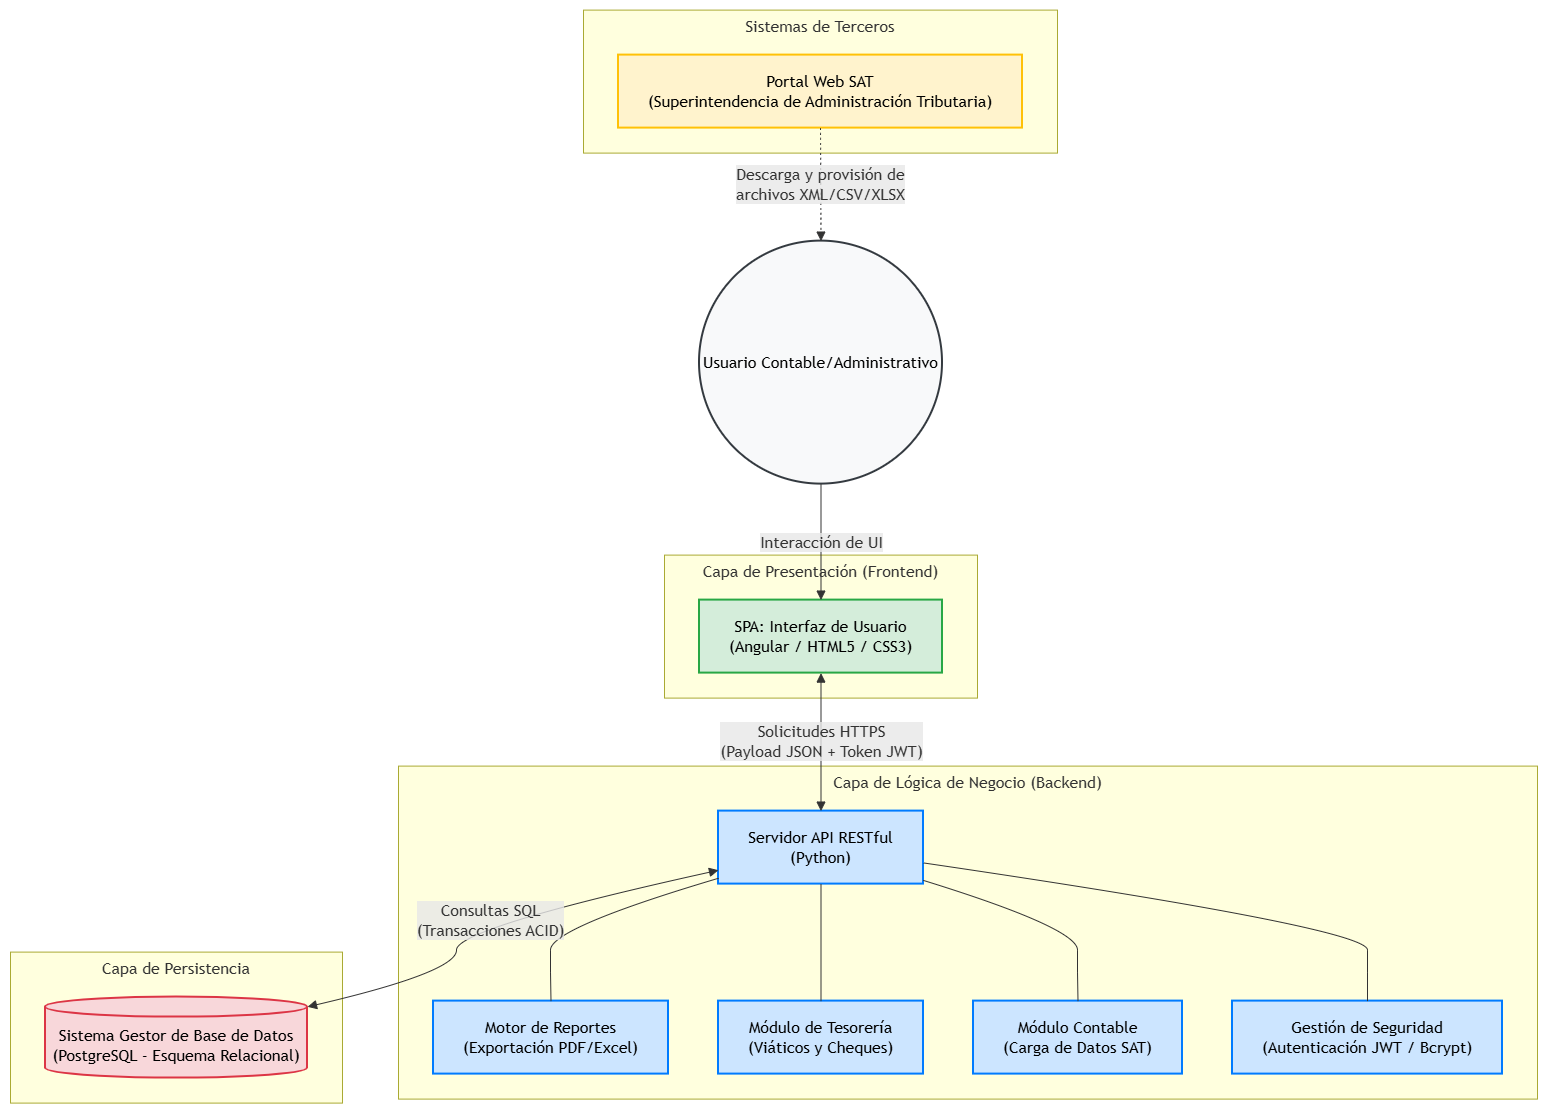
\includegraphics[width=0.92\linewidth]{imagenes/Arquitectura.png}
    \caption*{Nota. Elaboración propia con base en la arquitectura definida para el proyecto.}
\end{figure}

\subsubsection{Módulos funcionales}

\begin{longtable}{p{0.24\linewidth}p{0.68\linewidth}}
\textbf{Módulo} & \textbf{Responsabilidad técnica} \\
Login & Autenticar al usuario, emitir el token de sesión y aplicar permisos por rol. \\
Facturas FEL/SAT & Recibir XML o Excel, validar estructura, detectar duplicados, guardar comprobantes y permitir clasificación contable. \\
Cheques & Registrar cliente, bancos, fechas, estado, recepción de rechazo y asignación de factura. \\
Caja chica & Llamar facturas FEL por número, registrar recibos, controlar movimientos, aplicar nomenclatura y generar partidas. \\
Viáticos & Administrar colaboradores, territorios, giras, semanas, categorías, facturas, bonos y partidas semanales o transitorias. \\
Proveedores & Registrar NIT, crédito, retenciones, descuentos, cartera y partidas dentro del mes o transitorias. \\
Calendario & Consultar vencimientos, pagos, depósitos, cheques, giras y actividades. \\
Nomenclatura & Administrar código, nombre, naturaleza y estado de las cuentas contables. \\
Reportes & Consultar indicadores, filtros por período y exportaciones autorizadas. \\
\end{longtable}

\subsubsection{Diseño de la base de datos}
El modelo debe separar catálogos, documentos operativos y resultados contables. Las entidades principales son \texttt{usuarios}, \texttt{roles}, \texttt{permisos}, \texttt{proveedores}, \texttt{colaboradores}, \texttt{territorios}, \texttt{cuentas\_contables}, \texttt{bancos}, \texttt{facturas}, \texttt{cheques}, \texttt{movimientos\_caja\_chica}, \texttt{recibos}, \texttt{giras}, \texttt{liquidaciones\_viaticos}, \texttt{asignaciones\_facturas}, \texttt{partidas\_contables}, \texttt{detalles\_partida} y \texttt{auditoria\_eventos}.

Proveedor se relaciona con Factura y puede tener una cuenta contable asociada. Una Factura puede asignarse exclusivamente a Caja chica o Viáticos. Cheque se relaciona con Cliente, bancos, factura y recibo. Colaborador puede tener varios Territorios y una Gira selecciona un territorio y una semana. Partida contable contiene múltiples Detalles de partida, cada uno con cuenta, naturaleza, Debe y Haber.

Las tablas deben utilizar identificadores UUID o enteros autogenerados, fechas con zona horaria cuando corresponda, campos monetarios con tipo NUMERIC(14,2), estados controlados y restricciones de integridad. Las operaciones de generación de partidas deben ejecutarse dentro de transacciones PostgreSQL y verificar que el total del Debe sea igual al total del Haber.

\begin{figure}[H]
    \centering
    \caption{Modelo de base de datos PostgreSQL.}
    \label{fig:manual_tecnico_diagramabd}
    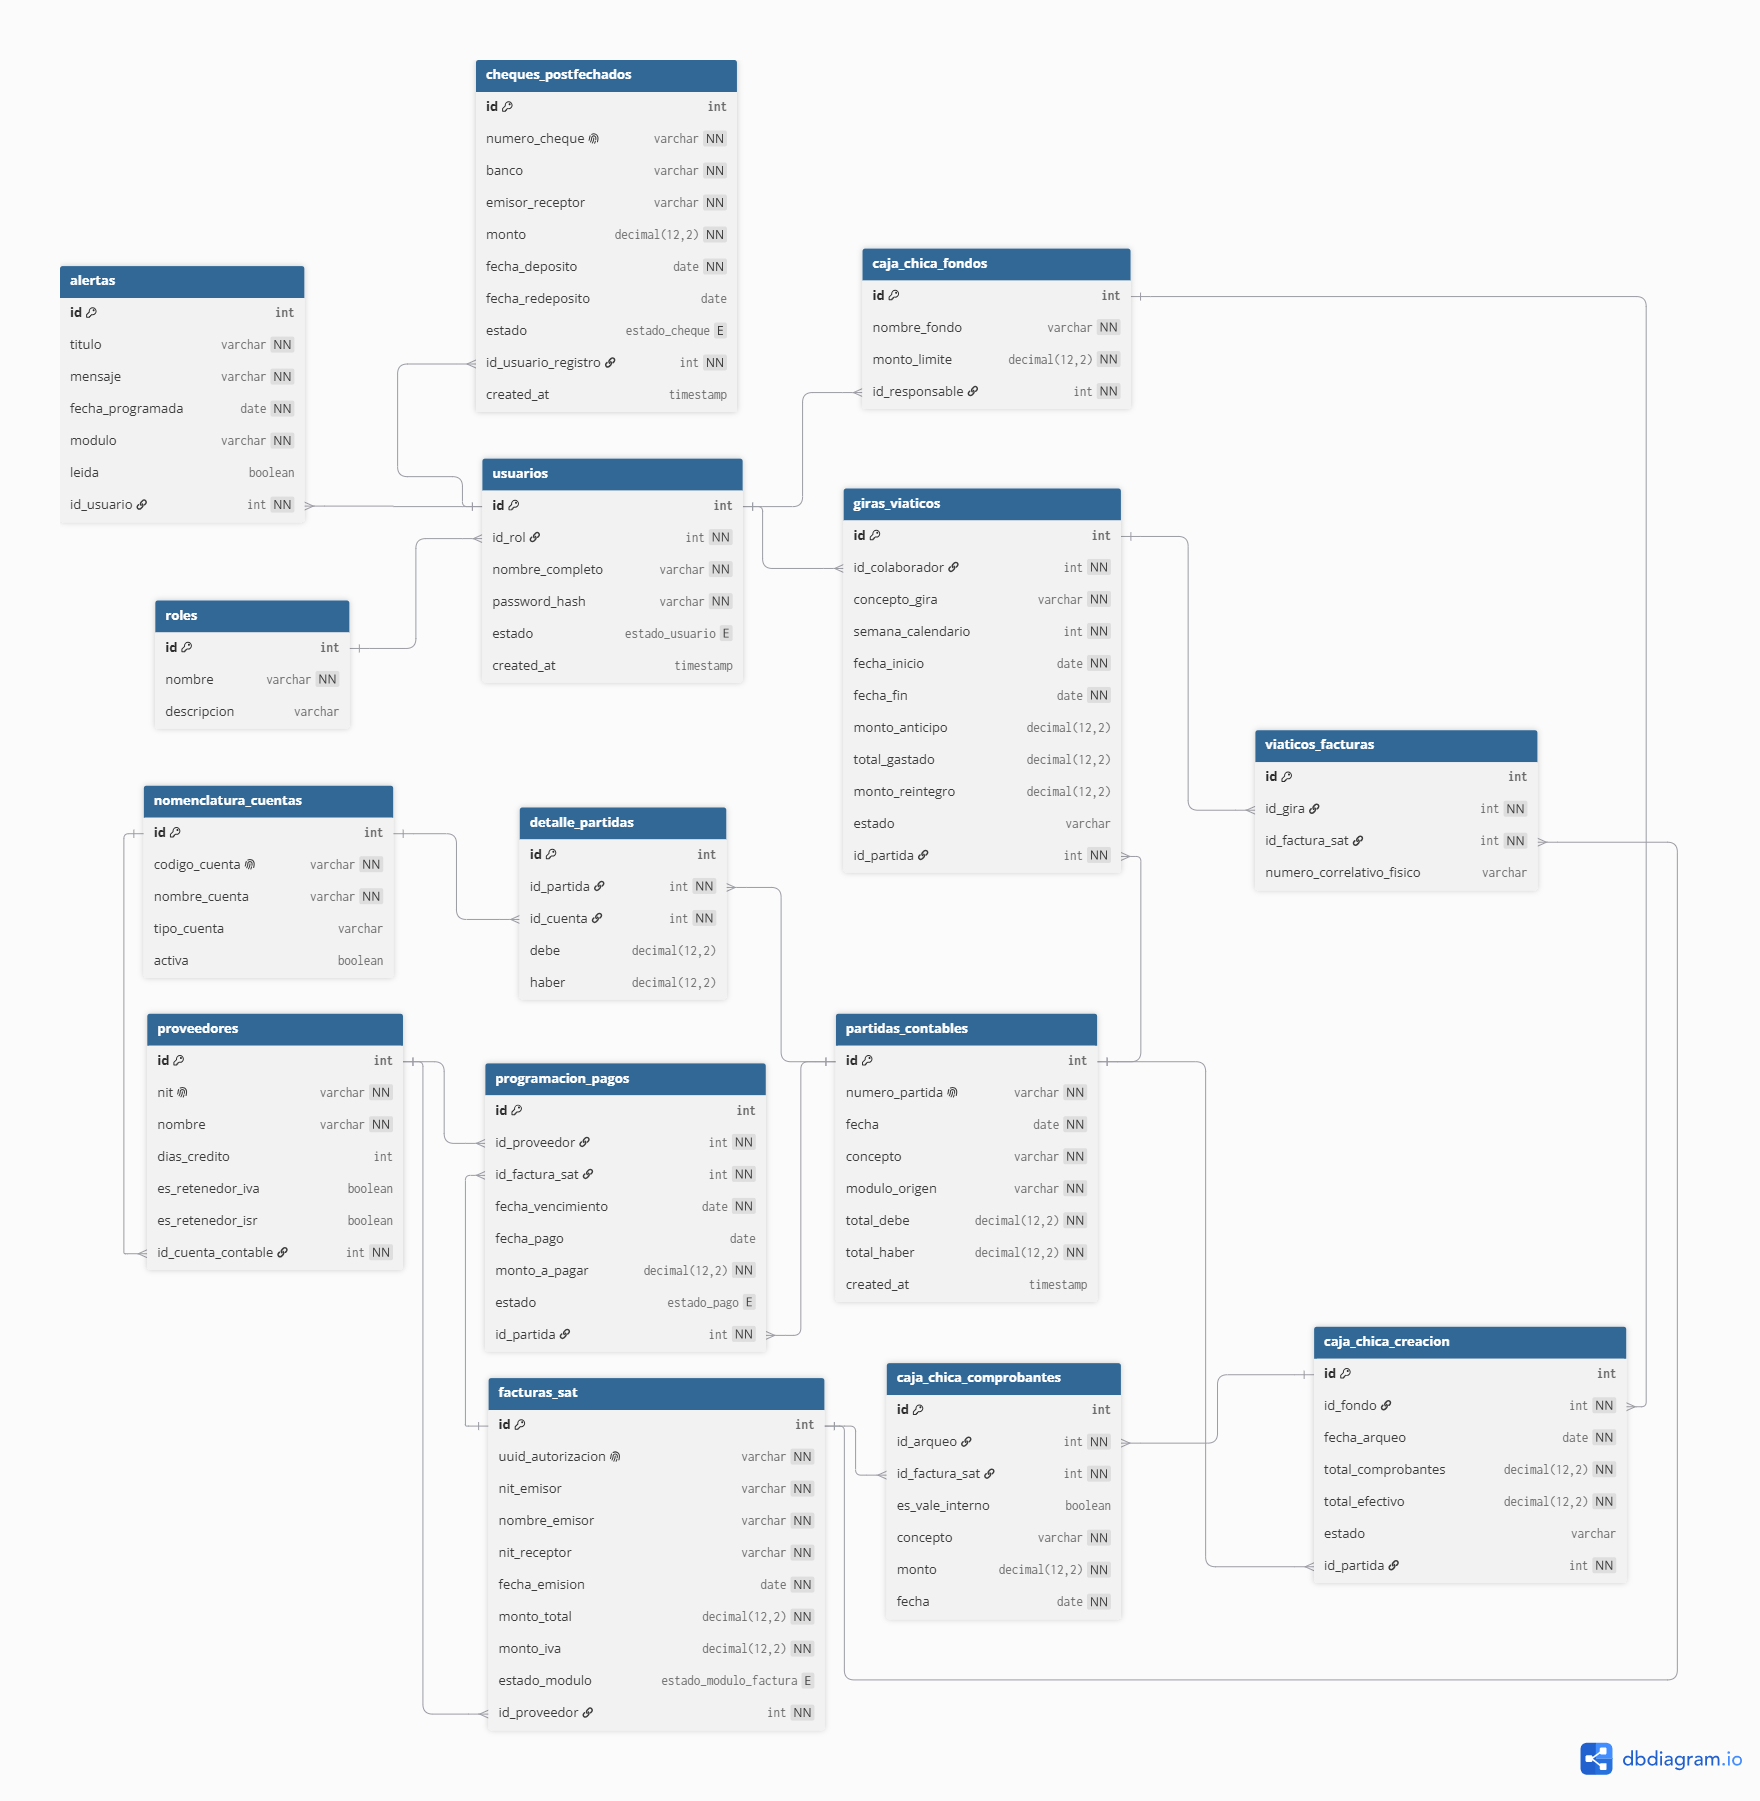
\includegraphics[width=0.92\linewidth]{imagenes/diagramabd.png}
    \caption*{Nota. Elaboración propia para el diseño de persistencia del Sistema Web.}
\end{figure}

\subsubsection{Reglas contables y de integridad}
La cuenta asignada al proveedor debe estar registrada en Nomenclatura. Cuando el sistema no reconoce automáticamente una factura por su descripción, combustible, lugar o concepto, el usuario debe seleccionar una cuenta contable válida del catálogo. La misma regla se aplica a Caja chica y Viáticos.

La generación dentro del mes utiliza Bancos como contrapartida cuando corresponde al pago del período. La partida transitoria utiliza Cuenta transitoria para documentos pendientes de pago. Retención ISR, Retención IVA y Otros descuentos deben conservarse como líneas independientes en el Haber. Las facturas ya asignadas no deben reutilizarse en otro módulo sin una operación autorizada de reversión.

\subsubsection{Tecnologías utilizadas}
La solución utiliza Angular para el frontend, Python para el backend y PostgreSQL para la persistencia. Angular organiza la interfaz como una aplicación de una sola página; Python expone la API y concentra la lógica de negocio; PostgreSQL mantiene la integridad, trazabilidad y consistencia de los datos contables. Las dependencias y versiones exactas deben mantenerse documentadas en los archivos de configuración del proyecto.

\subsubsection{Estructura del proyecto}

\begin{verbatim}
frontend-angular/
  src/app/
    core/                 # autenticación, guards e interceptores
    shared/               # componentes, pipes y validadores
    layout/               # menú lateral y barra superior
    modules/
      login/
      facturas-fel/
      cheques/
      caja-chica/
      viaticos/
      proveedores/
      calendario/
      nomenclatura/
      reportes/
    app-routing.module.ts

backend-python/
  app/
    api/                  # routers REST
    core/                 # configuración y seguridad
    models/               # modelos SQLAlchemy
    schemas/              # esquemas Pydantic
    services/             # reglas de negocio
    repositories/         # acceso a PostgreSQL
    migrations/           # Alembic
    main.py

base-datos/
  migrations/
  seeds_controlados/

documentacion/
  manuales/
  capitulos/
\end{verbatim}

\subsubsection{API y autenticación}
Los endpoints deben versionarse, por ejemplo, bajo \texttt{/api/v1}. El inicio de sesión devuelve un token JWT de corta duración y el frontend lo envía mediante un interceptor HTTP. Los guards de Angular restringen rutas y el backend vuelve a validar el rol; nunca se debe confiar únicamente en las restricciones de la interfaz.

Los endpoints deben validar tipos, campos obligatorios, permisos y estados de negocio. Las respuestas deben utilizar códigos HTTP coherentes, mensajes sin información sensible y un identificador de correlación para facilitar el diagnóstico. Las cargas de archivos deben limitar tamaño, extensión y contenido, y deben analizarse antes de procesarse.

\subsubsection{Configuración del entorno}
Para desarrollo se requiere Python 3.11 o la versión institucional aprobada, Node.js compatible con Angular, PostgreSQL, un entorno virtual de Python y las dependencias del proyecto. Las variables de entorno deben incluir la URL de PostgreSQL, secreto JWT, duración del token, configuración CORS y parámetros de almacenamiento.

Ejemplo de preparación del backend:

\begin{verbatim}
python -m venv .venv
source .venv/bin/activate
pip install -r requirements.txt
alembic upgrade head
uvicorn app.main:app --reload
\end{verbatim}

Ejemplo de preparación del frontend:

\begin{verbatim}
npm install
ng serve
ng build --configuration production
\end{verbatim}

Las claves y contraseñas deben permanecer fuera del repositorio. Para producción, el servidor debe usar HTTPS, variables protegidas y un usuario de PostgreSQL con los permisos mínimos necesarios.

\subsubsection{Despliegue}
El backend Python debe ejecutarse detrás de un servidor ASGI y un proxy inverso con HTTPS. El frontend Angular compilado debe publicarse como archivos estáticos o mediante el hosting institucional. Las rutas de Angular deben redirigir a \texttt{index.html}. PostgreSQL debe ubicarse en una red protegida, con respaldos automáticos, monitoreo y control de conexiones.

Antes de publicar se debe ejecutar una migración en un entorno de prueba, verificar login, importación FEL, asignación exclusiva, generación de partidas, exportación de reportes y recuperación ante errores. No se deben usar datos de demostración en el ambiente productivo.

\subsubsection{Mantenimiento preventivo y correctivo}
El mantenimiento preventivo incluye actualizar dependencias con control de versiones, revisar logs, aplicar migraciones, comprobar índices y validar respaldos. El mantenimiento correctivo debe reproducir el incidente, registrar módulo, usuario, fecha y operación, corregir la causa y ejecutar pruebas de regresión.

Los respaldos de PostgreSQL deben incluir al menos una copia completa y copias del esquema. Se debe comprobar periódicamente la restauración en un ambiente separado. Las operaciones destructivas sobre facturas, cheques, movimientos y partidas deben requerir autorización y conservar una entrada de auditoría.

\subsubsection{Evidencias visuales}
Las capturas incorporadas al paquete fueron tomadas del prototipo navegable y se conservan en la carpeta de imágenes. Las versiones anotadas del Manual de Usuario agregan números rojos y recuadros para explicar cada control. Las láminas agrupadas de componentes se mantienen como material complementario del Capítulo III.

\begin{figure}[H]
    \centering
    \caption{Componentes visuales agrupados del sistema.}
    \label{fig:manual_tecnico_elementos_04_tablas_tarjetas}
    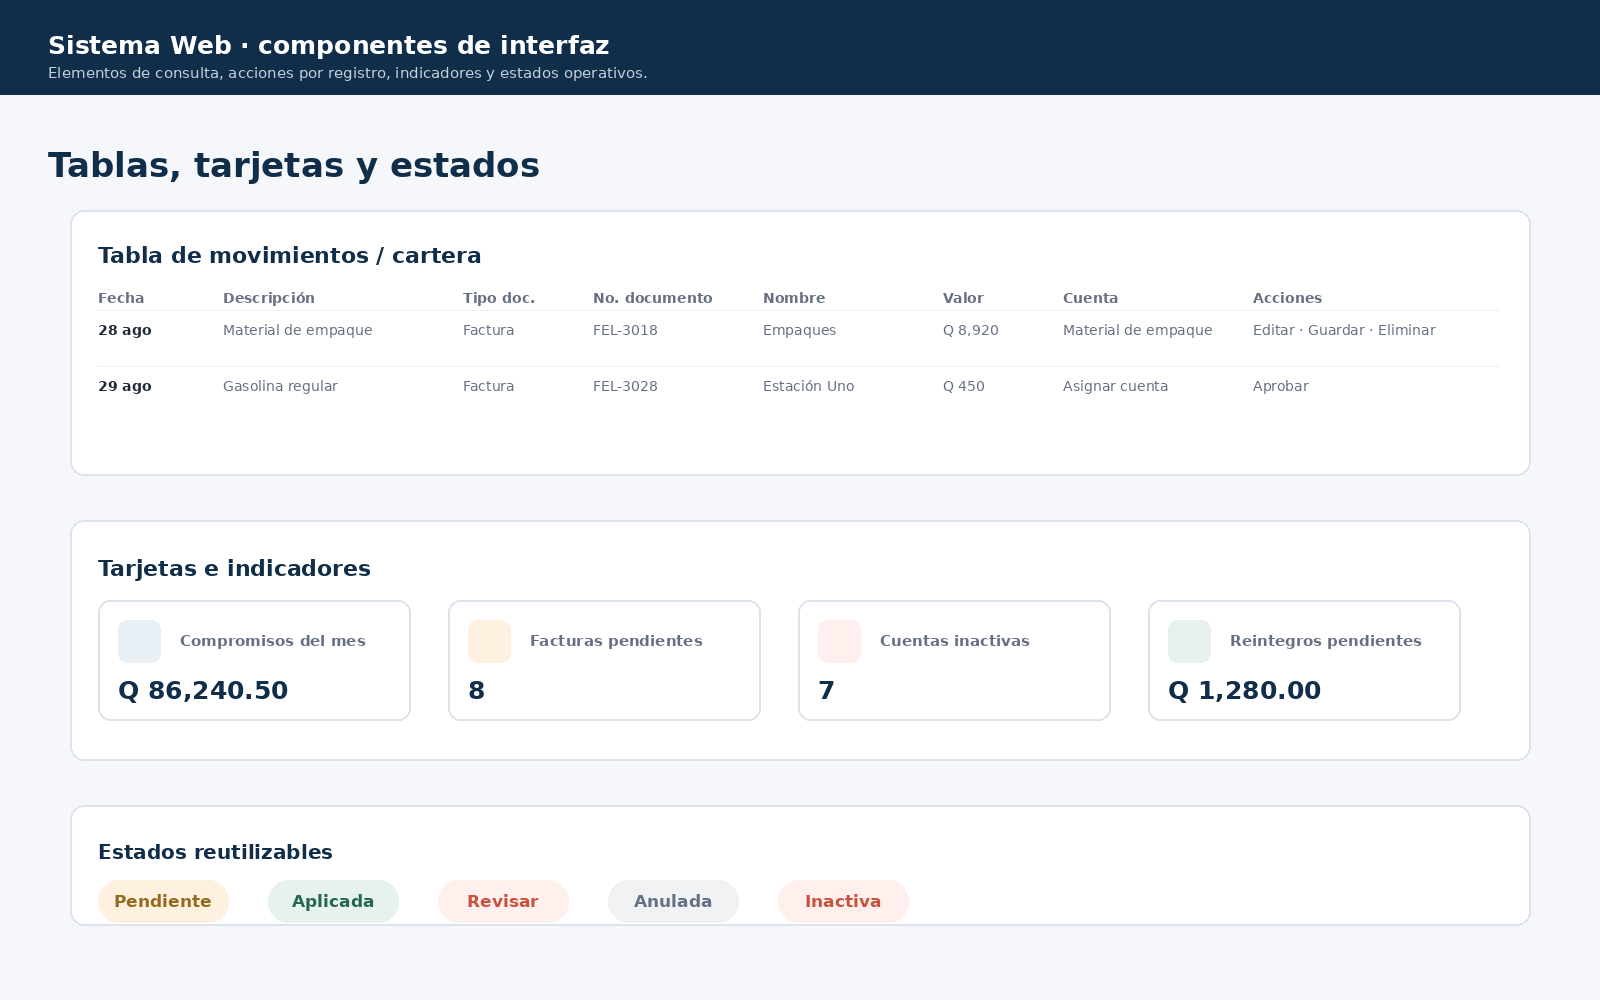
\includegraphics[width=0.92\linewidth]{imagenes/elementos_04_tablas_tarjetas.png}
    \caption*{Nota. Elaboración propia a partir de los componentes del prototipo.}
\end{figure}

\subsubsection{Matriz mínima de pruebas técnicas}

\begin{longtable}{p{0.25\linewidth}p{0.34\linewidth}p{0.29\linewidth}}
\textbf{Módulo} & \textbf{Prueba} & \textbf{Resultado esperado} \\
Login & Credenciales válidas e inválidas & Acceso autorizado o mensaje controlado. \\
FEL/SAT & XML duplicado o con error & Rechazo, aviso y conservación de trazabilidad. \\
Cheques & Cambio de estado y asignación & Estado, fechas y detalle de factura consistentes. \\
Caja chica & Movimiento sin cuenta reconocida & Solicitud de clasificación manual desde Nomenclatura. \\
Viáticos & Partida semanal y transitoria & Debe y Haber balanceados y documentos no duplicados. \\
Proveedores & Vencido y pendiente de pago & Selección correcta entre Bancos y Cuenta transitoria. \\
Nomenclatura & Cuenta Debe/Haber activa o inactiva & Validación de naturaleza y disponibilidad. \\
Reportes & Filtro y exportación & Información correspondiente al período seleccionado. \\
\end{longtable}


\subsubsection{Acceso e instalación}
La instalación se realiza en tres capas. Primero se prepara el entorno del frontend Angular y se instalan sus dependencias. Después se configura el servicio backend desarrollado en Python y sus variables de entorno. Finalmente se crea la base de datos PostgreSQL, se aplican las migraciones y se verifica la conexión entre las capas.

\subsubsection{Configuración por ambientes}
El proyecto debe separar los ambientes de desarrollo, pruebas y producción. Cada ambiente debe utilizar sus propias credenciales, URL de conexión y parámetros de seguridad. Las claves de acceso no deben almacenarse dentro del código fuente ni incorporarse al repositorio.

\subsubsection{Respaldo y recuperación}
El responsable técnico debe programar respaldos de PostgreSQL, verificar periódicamente que los archivos puedan restaurarse y documentar la fecha, responsable y resultado de cada prueba. Antes de una actualización, debe realizarse un respaldo completo y conservarse una copia fuera del servidor principal.

\subsubsection{Lista de verificación de mantenimiento}
El mantenimiento incluye actualizar dependencias de Angular y Python, revisar logs, verificar tareas programadas, comprobar el espacio disponible de PostgreSQL, validar permisos y ejecutar las pruebas funcionales de los módulos FEL/SAT, Cheques, Caja chica, Viáticos, Proveedores, Nomenclatura y Reportes.

\subsubsection{Pruebas técnicas mínimas}
\begin{longtable}{p{3.5cm}p{7.5cm}p{3cm}}
\caption{Pruebas técnicas mínimas del sistema}\label{tab:B_pruebas_tecnicas}\\
\toprule
\textbf{Prueba} & \textbf{Resultado esperado} & \textbf{Responsable}\\
\midrule
Conexión a PostgreSQL & El backend establece conexión y registra el resultado sin exponer credenciales. & Técnico\\
Autenticación & Angular envía la solicitud al backend Python y recibe una respuesta controlada. & Técnico\\
Importación FEL & El sistema valida el archivo y evita duplicados. & Auxiliar\\
Partida contable & Debe y Haber coinciden antes de guardar el registro. & Contador\\
Respaldo & La copia puede restaurarse en un ambiente de prueba. & Técnico\\
\bottomrule
\end{longtable}

\subsubsection{Anexos técnicos}
Los anexos técnicos comprenden el diagrama de arquitectura, el modelo de datos PostgreSQL, la matriz mínima de pruebas y las capturas de referencia del sistema. Estos anexos respaldan la explicación técnica y deben mantenerse sincronizados con los cambios aprobados en Angular, Python y PostgreSQL.
